\documentclass{article}
\usepackage{graphicx}
\usepackage{amsmath}
\usepackage[margin=2cm]{geometry}

\title{HybridSort Analysis: Optimal \( K \) and Comparison Counts for Random and Sorted Arrays}
\author{}
\date{\today}

\begin{document}

\maketitle

\section{Atrribution: }
\textbf{\textit{This project is made from scratch.}}

\section{Implemention code of Hybrid Sort (Deliverable 1): }
\begin{verbatim}
    def hybrid_sort(array, k):
    n = len(array)
    if n <= k:
        insertion_sort(array, 0, n - 1)
    else:
        mid = n // 2
        left, right = array[:mid], array[mid:]
        hybrid_sort(left, k)
        hybrid_sort(right, k)
        array[:] = merge(left, right)
\end{verbatim}

The correctness of the algorithm is demonstrated in the output of the code. 
\section{Results and Analysis}

\subsection{Random Arrays}
The average comparison counts for random arrays across varying \( K \) values show that:
\begin{itemize}
    \item Lower \( K \) values perform better consistently: For all tested sizes, \( K = 5 \) yields the lowest average comparisons. This suggests that smaller subarrays benefit from Insertion Sort due to its efficiency on short lists, especially when the input order is highly irregular, as with random arrays.
    \item Increased \( K \) values lead to higher comparisons: As \( K \) increases, HybridSort engages Insertion Sort over larger subarrays, reducing the effectiveness of Merge Sort. This is particularly noticeable in larger arrays, where \( K = 99 \) leads to significantly higher comparison counts, indicating that Merge Sort’s efficiency is better leveraged with a smaller \( K \) threshold.
\end{itemize}

These findings imply that for random arrays, a low \( K \) value is preferable across all sizes, as seen in Figure~\ref{fig:random_comparisons}, where \( K = 5 \) consistently minimizes comparisons for arrays up to 10,000 elements.

\begin{figure}[!ht]
    \centering
    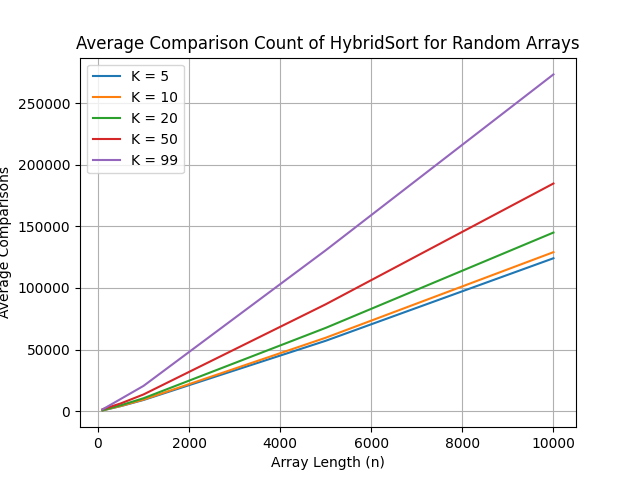
\includegraphics[width=0.8\textwidth]{../average_comparisons_random.png}
    \caption{Average Comparisons for HybridSort on Random Arrays with Different \( K \) Values}\label{fig:random_comparisons}
\end{figure}

\subsection{Sorted Arrays}
For sorted arrays, we observe a different trend:
\begin{itemize}
    \item Higher \( K \) values minimize comparison : As \( K \) increases, the average number of comparisons decreases, particularly for larger array sizes. For \( n = 5000 \) and \( n = 10000 \), \( K = 99 \) results in the fewest comparisons, indicating that larger subarrays benefit from using Insertion Sort directly when elements are nearly sorted.
    \item Reduced overhead in sorted data: With sorted data, Insertion Sort encounters minimal shifting requirements, making it more efficient than Merge Sort. Therefore, increasing \( K \) to 99 avoids unnecessary recursion and leverages Insertion Sort’s efficiency on already ordered data.
\end{itemize}

These findings suggest that for sorted arrays, larger \( K \) values are preferable, as shown in Figure~\ref{fig:sorted_comparisons}. The graph illustrates that as array size grows, the benefit of using Insertion Sort directly on large segments becomes more pronounced.

\begin{figure}[!ht]
    \centering
    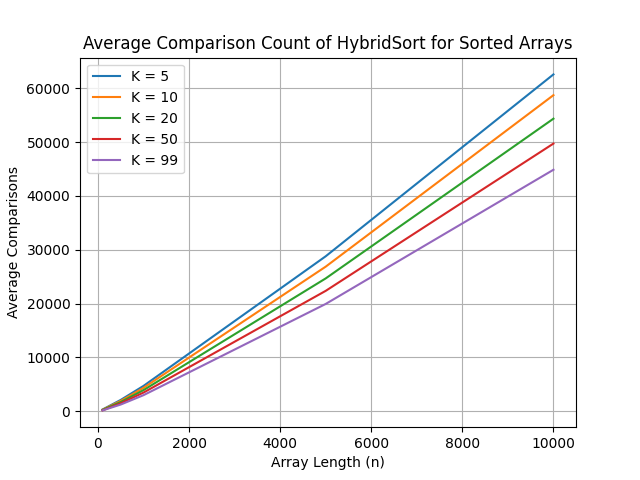
\includegraphics[width=0.8\textwidth]{../average_comparisons_sorted.png}
    \caption{Average Comparisons for HybridSort on Sorted Arrays with Different \( K \) Values}\label{fig:sorted_comparisons}
\end{figure}

\subsection{Optimal \( K \) Selection}
The optimal \( K \) value for random arrays remains consistently low (specifically \( K = 5 \)) across all array sizes, while for sorted arrays, the optimal \( K \) shifts to the highest tested values, with \( K = 99 \) being consistently optimal for arrays of size 500 and above. This highlights that:
\begin{itemize}
    \item Random arrays benefit from smaller \( K \), as smaller subarrays allow HybridSort to capitalize on Merge Sort’s divide-and-conquer efficiency.
    \item Sorted arrays benefit from larger \( K \), allowing Insertion Sort to perform the final sorting efficiently without further partitioning.
\end{itemize}
s
Figures~\ref{fig:optimal_k} and~\ref{fig:optimal_k_sorted} summarizes the optimal \( K \) values for both array types across sizes.

\begin{figure}[!ht]
    \centering
    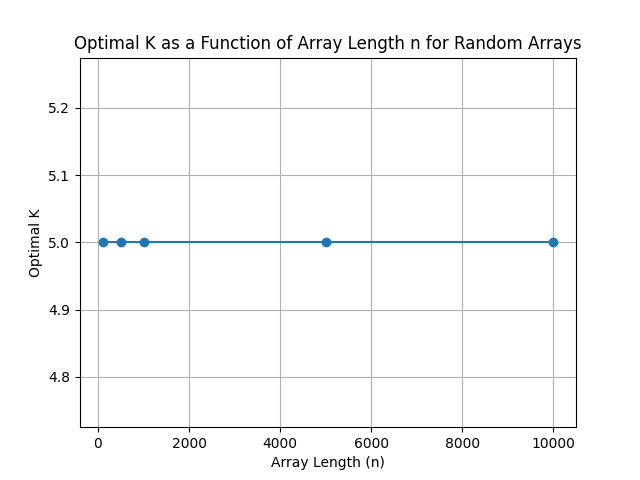
\includegraphics[width=0.8\textwidth]{../optimal_k_comparisons_random.png}
    \caption{Optimal \( K \) Values as a Function of Array Length \( n \) for Random and Sorted Arrays}\label{fig:optimal_k}
\end{figure}

\begin{figure}[!ht]
    \centering
    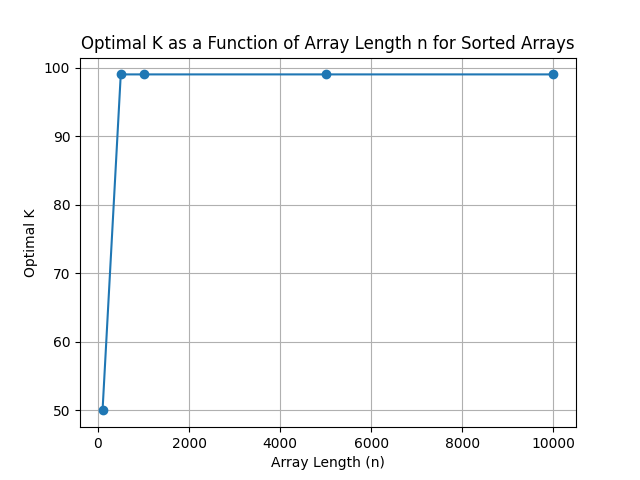
\includegraphics[width=0.8\textwidth]{../optimal_k_comparisons_sorted.png}
    \caption{Optimal \( K \) Values as a Function of Array Length \( n \) for Sorted Arrays}\label{fig:optimal_k_sorted}
\end{figure}
\section{Conclusion}
After Analysis of the graphs over numerous iterations, I see that the hybrid sort is influenced heavily by the selection of k. 
\begin{itemize}
    \item Random Array: A smaller \( K \) (specifically, \( K = 5 \)) is consistently optimal, allowing Merge Sort to handle most of the array while using Insertion Sort on minimal segments.
    \item Sorted Array: it is reverse for sorted arryass. Larger \( K \) values (e.g., \( K = 99 \)) minimize comparisons, leveraging Insertion Sort’s reduced overhead on preordered data. I also saw that the maximum K we can have on sorted arrrays is at most of half the size of array. If the n is relatively very large thann k then maximum k value yeilds the fastest possible sort process. We can see more of that on console output. 
\end{itemize}

\end{document}
